%%%%%%%%%%%%%%%%%%%%%%%%%%%%%%%%%%%%%%%%%%%%%%%%%%%%%%%%%%%%%%%%%%%%%%%%%%

% abnTeX2: Modelo de Trabalho Acadêmico em conformidade com 
% as normas da ABNT

%%%%%%%%%%%%%%%%%%%%%%%%%%%%%%%%%%%%%%%%%%%%%%%%%%%%%%%%%%%%%%%%%%%%%%%%%%

\documentclass[english, 
               brazil, 
               bsc] %Opções bsc (TCC) e msc (Mestrado)
               {dcomp-abntex2}


%%%%%%%%%%%%%%%%%%%%%%%%%%%%%%%%%%%%%%%%%%%%%%%%%%%%%%%%%%%%%%%%%%%%%%%%%%
% Área para adição de pacotes extras
%%%%%%%%%%%%%%%%%%%%%%%%%%%%%%%%%%%%%%%%%%%%%%%%%%%%%%%%%%%%%%%%%%%%%%%%%%

\usepackage{lipsum} % Retirar para a versão final do documento
\usepackage{float}
\restylefloat{table}

%Utilize aqui seu pacote preferido para algoritmos
\usepackage[linesnumbered]{algorithm2e}

%%%%%%%%%%%%%%%%%%%%%%%%%%%%%%%%%%%%%%%%%%%%%%%%%%%%%%%%%%%%%%%%%%%%%%%%%%

%Compila o indice
\makeindex

\begin{document}

% Seleciona o idioma do documento (conforme pacotes do babel)
\selectlanguage{brazil}

% Retira espaço extra obsoleto entre as frases.
\frenchspacing 

%%%%%%%%%%%%%%%%%%%%%%%%%%%%%%%%%%%%%%%%%%%%%%%%%%%%%%%%%%%%%%%%%%%%%%%%%%
% ELEMENTOS PRÉ-TEXTUAIS
%%%%%%%%%%%%%%%%%%%%%%%%%%%%%%%%%%%%%%%%%%%%%%%%%%%%%%%%%%%%%%%%%%%%%%%%%%

\pretextual


\titulo{Desenvolvimento de um Compilador de BRDFs em LaTeX para linguagem de shading GLSL, através da técnica Pratt Parsing } 
\autor{Everton Santos de Andrade Júnior}
\orientador{Beatriz Trinchão Andrade}
\coorientador{Gastao Florencio Miranda Junior}
\curso{Ciência da Computação}

\inserirInformacoesPDF

\imprimircapa
\imprimirfolhaderosto*

% \begin{dedicatoria}
   \vspace*{\fill}
   \centering
   \noindent
   \textit{Esta página foi deixada em branco, não-ironicamente, de propósito} \vspace*{\fill}
\end{dedicatoria}
% ---

% \include{Pre_Textual/Agradecimentos}
% \begin{epigrafe}[]
    \vspace*{\fill}
	\begin{flushright}
	
		\textit{Este trabalho, além de cultural, filosófico e pedagógico\\
				É também medicinal, preventivo e curativo\\
				Servindo entre outras coisas para pano branco e pano preto\\
				Curuba e ferida braba\\
				Piolho, chulé e caspa\\
				Cravo, espinha e berruga\\
				Panarismo e água na pleura\\
				Só não cura o velho chifre\\
				Por que não mata a raiz\\
				Pois fica ela encravada\\
				No fundo do coração\\
				(Falcão)}
		
	\end{flushright}
\end{epigrafe}
% ---

% resumo em português
\setlength{\absparsep}{18pt} % ajusta o espaçamento dos parágrafos do resumo
\begin{resumo}
 
% Segundo a \citeonline[3.1-3.2]{NBR6028:2003}, o resumo deve ressaltar o objetivo, o método, os resultados e as conclusões do documento. A ordem e a extensão destes itens dependem do tipo de resumo (informativo ou indicativo) e do tratamento que cada item recebe no documento original. O resumo deve ser precedido da referência do documento, com exceção do resumo inserido no próprio documento. (\ldots) As palavras-chave devem figurar logo abaixo do resumo, antecedidas da expressão Palavras-chave:, separadas entre si por ponto e finalizadas também por ponto.


  O presente trabalho propõe o desenvolvimento de um compilador de funções de distribuição de reflexão bidirecional (BRDFs) expressas em \LaTeX{}  para a linguagem de \textit{shading} GLSL, utilizando a técnica de Pratt \textit{Parsing} e linguagem de programação Odin.
  O objetivo é automatizar o processo de tradução de funções complexas de materiais, descritas em equações \LaTeX{}, para o código GLSL utilizado na programação de \textit{shaders} para OpenGL.
  Ao fornecer essa ferramenta, pretende-se não apenas simplificar o trabalho dos desenvolvedores e pesquisadores na área de computação gráfica, mas também democratizar o acesso e compreensão de modelos de materiais complexos. Além disso, ao permitir que as BRDFs sejam expressas em uma forma mais familiar e acessível, como a notação matemática, o compilador reduz a barreira de entrada para aqueles que não estão familiarizados com linguagens programação, de modo a facilitar a colaboração interdisciplinar entre profissionais de diferentes áreas. A validação dos \textit{shaders} de saída do compilador proposto será feita através da ferramenta Disney BRDF Explorer, que possibilita a visualização e análise de BRDFs.

  \textbf{Palavras-chave}: Compilador, BRDFs, LaTeX, GLSL, Shading, Pratt \textit{Parsing}.
\end{resumo}

% \include{Pre_Textual/Abstract}


\mostrarlistadeILUSTRACOES
\mostrarlistadeQUADROS
\mostrarlistadeTABELAS
% \mostrarlistadeCODIGOS
% \mostrarlistadeALGORITMOS
 
\include{Pre_Textual/Abreviaturas}
% % ---
% inserir lista de símbolos
% ---

\begin{simbolos}
  \item[$ \Gamma $] Letra grega Gama
  \item[$ \Lambda $] Lambda
  \item[$ \zeta $] Letra grega minúscula zeta
  \item[$ \in $] Pertence
\end{simbolos}
% ---

    
\mostrarSUMARIO

%%%%%%%%%%%%%%%%%%%%%%%%%%%%%%%%%%%%%%%%%%%%%%%%%%%%%%%%%%%%%%%%%%%%%%%%%%
% ELEMENTOS TEXTUAIS
%%%%%%%%%%%%%%%%%%%%%%%%%%%%%%%%%%%%%%%%%%%%%%%%%%%%%%%%%%%%%%%%%%%%%%%%%%

\textual

%%%%%%%%%%%%%%%%%%%%%%%%%%%%%%%%%%%%%%%%%%%%%%%%%%%%%%%%%%%%%%%%%%%%%%%%%%
% Introdução
%%%%%%%%%%%%%%%%%%%%%%%%%%%%%%%%%%%%%%%%%%%%%%%%%%%%%%%%%%%%%%%%%%%%%%%%%%
\chapter{Introdução}


\section{Contexto}

Na computação gráfica, a representação realista de cenas tridimensionais depende fortemente da modelagem da luz. A interação da luminosidade incidente no objeto, bem como os materiais que compõem esses objetos, são aspectos críticos a serem considerados na geração dessas cenas [referencia]. Na prática, essa interação é frequentemente modelada por meio de funções de distribuição de refletância bidirecional, conhecidas como BRDFs.


As BRDFs, essencialmente, calculam a proporção entre a energia luminosa que atinge um ponto na superfície e como essa energia é refletida, transmitida ou absorvida [referencia]. Na renderização, essas funções são implementadas por meio programas especializados das unidades de processamento gráfico (GPUs), esses programmas são chamados de shaders, e cada API de rederização disponibiliza etapas diferentes onde esses executaveis podem ser mudados durante o processo de renderização. Esses shaders concedem a capacidade de cada objeto renderizado ter sua aparência configurada por meio de um código que implementa uma BRDF.


\section{Motivação}

Apesar da disponibilidade de linguagens específicas para a programação de shaders, que possibilitam a modificação procedimentos que representam uma BRDF, a aplicação de BRDFs na geração de shaders requer conhecimento especializado em programação [referencia?]. Essa barreira técnica pode restringir a exploração dos efeitos visuais por profissionais de áreas não relacionadas à programação. Diante disso, surge a necessidade de ferramentas mais acessíveis para a criação de shaders.

No meio acadêmico, as BRDFs são, comumente, descritas por uma fórmula escrita em LaTeX, uma abordagem promissora para atender a essa necessidade é o desenvolvimento de um compilador capaz de traduzir BRDFs em LaTex para shaders, assim democratizando a visualização dessas BRDFs. Dado que as fórmulas são equações matemáticas, precisamos retrigir repretsentação da linguagem de entrada para o compilador afim de garatir um projeto útil em tempo ábil.

\section{Objetivo}
Este trabalho visa projetar e implementar um compilador que, a partir de funções de distribuição de refletância bidirecional escrita como equações em LaTeX, seja capaz de gerar código de shading na linguagem alvo da API OpenGL (referencia). A saída será um shader capaz de reproduzir as características de reflexão da função de refletância original, considerando a precedencia de operadores, em uma superfície tridimensional, ou, ao menos, alcançar uma aproximação satisfatória dessas características, considerando as limitações da linguagem de shading da API principalmente as representações de dados de forma discreta.

\section{Metodologia}
Para alcançar o objetivo, a sequencia das etapas adotadas serão as seguintes.


\begin{enumerate}

   \item Realizar uma análise abrangente das áreas relacionadas ao desenvolvimento da ferramenta proposta;
   \item Investigar o estado da arte no campo da compilação de BRDFs em linguagens de shading;
   \item Definir a linguagem de entrada e a linguagem de saída do compilador;
   \item Elaborar testes com equações LaTeX de entrada pareado com a saída em shader GLSL esperado;
   \item Implementar o compilador utilizando uma linguagem de programação e tecnicas recursivas de parsing
   \item Realizar a renderização de cenas utilizando o shader gerado pelo compilador.

\end{enumerate}

% Apesar da importância de usar técnicas confiáveis para avaliar um BRDF, há uma falta de trabalhos na literatura que reúnam e comparem essas técnicas.
% Este artigo propõe uma compilação de técnicas usadas para avaliar representações de BRDF, juntamente com suas definições formais. Essas técnicas foram classificadas em três grupos diferentes - funções de comparação, imagens renderizadas e gráficos - e, para ilustrar seu uso, três modelos clássicos e amplamente adotados e uma representação de BRDF de ponta foram avaliados quanto à sua capacidade de preservar a aparência de materiais medidos. Com base em nossa pesquisa sobre funções de comparação, uma técnica de avaliação de BRDF estável e robusta é proposta. Observou-se tanto durante a revisão da literatura quanto nos experimentos que cada grupo de técnicas fornece informações complementares sobre os BRDFs avaliados, o que sugere que pelo menos um modelo de cada categoria deve ser adotado durante a escolha de critérios para avaliar um BRDF.

%%%%%%%%%%%%%%%%%%%%%%%%%%%%%%%%%%%%%%%%%%%%%%%%%%%%%%%%%%%%%%%%%%%%%%%%%%
% Revisão Bibliográfica 
%%%%%%%%%%%%%%%%%%%%%%%%%%%%%%%%%%%%%%%%%%%%%%%%%%%%%%%%%%%%%%%%%%%%%%%%%%
\chapter{Revisão Bibliográfica}

Para esta seção, será conduzida uma revisão literária abrangente com o objetivo de explorar trabalhos relacionados ao desenvolvimento de compiladores para tradução de BRDFs expressas em LaTeX para a linguagem de shading, empregando, técnicas de parsing. O processo de busca será conduzido em duas etapas distintas. Primeiramente, será realizado um levantamento dos trabalhos existentes nas bases de dados  com relevantes periodicos, anais de eventos, artigos e trabalhos. 


Por fim, será realizada uma busca por produtos ou ferramentas similares no mercado, utilizando strings de busca específicas em repositórios digitais, especificamente GitHub, e SourceForge. Esses processos de busca permitirão identificar referências relevantes e estabelecer um panorama do estado da arte no campo dos compiladores de BRDFs  para shaders, contribuindo para a compreensão do contexto acadêmico e prático no qual este trabalho se insere.

\section{Mapeamento Sistemático}

Com o intuito de obter resultados relevantes para a pesquisa, foram elaboradas frases de busca com base nos termos-chave relacionados ao tema deste trabalho. Assim como, foram criadas questões de pesquisa para guiar a seleção dos trabalhos.

\subsection{Seleção das Bases}
As bases escolhidas foram: ACM Digital Library,  IEEE Xplorer Digital Library,  Biblioteca Digital Brasileira de Teses e Dissertações (BDTD), Portal de Periódicos da CAPES,  Google Acadêmico, esse foram escolhidos por serem acessíveis gratuitamente pela afiliação à Universidade Federal de Sergipe, já o google scholar foi escolhido para agregar pesquisas em outras bases que possam ter trabalhos relevantes.
\url{https://bdtd.ibict.br/}
\url{https://ieeexplore.ieee.org/}
\url{https://www-periodicos-capes-gov-br.ezl.periodicos.capes.gov.br/}



\subsection{Questões de Pequisa} \label{sec:questoes-pesquisa}

Foram elaboradas questões de pesquisa específicas, que guiam as frases-chave que refletem os principais aspectos do tema em questão. A partir desse processo, foram identificados e selecionados os trabalhos que melhor atendiam às questões propostas, garantindo maior relevância para o estudo em questão.

\begin{enumerate}
  \item Quais são as abordagens mais comuns utilizadas na criação de compiladores para tradução de BRDFs expressas em alguma linguagem de texto, com LaTeX, para shaders?

  \item Quais as técnicas de parsing que têm sido aplicadas no desenvolvimento de compiladores para linguagens matemáticas como LaTeX?

  \item O trabalho utiliza arvores, ou gramáticas livre de contexto para representar uma BRDF?

 \item Quais são os principais desafios enfrentados ao traduzir funções matemáticas complexas, como as BRDFs, em shaders?

 \item Quais são as ferramentas e recursos disponíveis para auxiliar no desenvolvimento de compiladores para BRDFs e shaders, e como elas podem ser integradas ao processo de desenvolvimento?

\end{enumerate}



\subsection{Termos de Busca}
 As frases foram contruidas considerando suas variações equivalentes através de operadores lógicos. Posteriormente, as frases de pesquisa foram adaptadas de acordo com as características individuais de cada base de dados utilizada nas pesquisas. Os termos-chave escolhidos foram: "shader", "BRDF", "compiler", "parser" e "grammar".


\begin{table}[H]
\ABNTEXfontereduzida
\caption[bases]{}
\label{tab-bases}
\begin{tabular}{p{2.6cm}|p{6.0cm}|p{2.25cm}|p{3.40cm}}
  %\hline
   \textbf{Bases} & \textbf{Termos de Pesquisa}  & \textbf{Resultados}\\
   \hline
    IEEE Xplore Digital Library
    &
    ("Full Text \& Metadata":brdf)
AND (("Full Text \& Metadata":shader) OR  ("Full Text \& Metadata":shading))
AND (("Full Text \& Metadata":compiler) OR  ("Full Text \& Metadata":parsing) OR  ("Full Text \& Metadata":parser) OR  ("Full Text \& Metadata":grammar))
   & 36
    \\ \hline

    BDTD
    & (Todos os campos:compiler OU Todos os campos:parsing OU Todos os campos:parser OU Todos os campos:compilador) E (Todos os campos:shader OU Todos os campos:shading) E (Todos os campos:brdf)
    & 0
    \\ \hline
    CAPES Periodico
    &  Qualquer campo contém brdf E 
 Qualquer campo contém compi* E shad*  
    & 0
    \\ \hline

  ACM Digital Library
  & AllField:((shader OR shading) AND brdf AND (compiler OR compiling) AND (parser OR grammar OR parsing))
  & 46
    \\ \hline

 Google Academico 
  & 
  ("BRDF" AND ("COMPILER" OR "COMPILING") AND( "PARSER" OR "PARSING") AND ("SHADER" OR "SHADING"))
  & 69
   % \hline
\end{tabular}
% \legend{Fonte: \citeonline{van86}}
\end{table}

\subsection{Critérios}

Para garantir relevancia dos resultados obtivos, seguimos os critérios de inclusão e exclusão estabelecidos, de forma que os resultados serão filtrados. Ao fim desse procedimento, apenas os resultados com maior compatibilidade com este trabalho seram análisado e descritos de maneira mais detalhada.

\subsubsection{Critérios de Inclusão}

\begin{enumerate}
  \item Foram incluídos artigos relacionados às palavras-chaves;
  \item Foram incluídos artigos que de alguma forma inclua a criação de um compilador ou um parser;
  \item Foram incluídos artigos que sintetize uma arvóre como representação de BRDFs
\end{enumerate}

\subsubsection{Critérios de Exclusão}

\begin{enumerate}
  \item Foram excluídos artigos dos quais dispunham de links incorretos e ou quebrados;
  \item Foram excluídos artigos que dispunham de aplicacões muito similares/repetitivas;
  \item Foram excluídos artigos que não respodem as questões de pesquisa \ref{sec:questoes-pesquisa};
  \item Artigo que não tem como entrada a BRDFs no formato de equação, ou seja, está utilizando a representação diretamente como código, também foi excluído.
  \item Foram excluídos artigos que não consideram a geração de shaders como saída ou estrutura da BRDF em arvore.
  \item Foram excluídos artigos que não citam BRDFs e compilador em seu resumo;
  \item Se após a leitura completa, o artigo não concerne os interesse deste trabalho, esse foi excluído.
\end{enumerate}


\begin{table}[H]
\ABNTEXfontereduzida
  \caption[bases]{Resultados da Base após aplicar os critérios}
\label{tab-bases}
\begin{tabular}{p{6.6cm}|p{6.6cm}}
  %\hline
   \textbf{Bases}  & \textbf{Filtrados}\\
   \hline
    IEEE Xplore Digital Library
   & 2
    \\ \hline
    BDTD
    & 0
    \\ \hline
    CAPES Periodico
    & 0
    \\ \hline

  ACM Digital Library
  & 1
    \\ \hline
 Google Academico 
  & 1
   % \hline
\end{tabular}
% \legend{Fonte: \citeonline{van86}}
\end{table}



\subsection{Descrição dos Trabalhos Relacionados}

\subsubsection{genBRDF: Discovering New Analytic BRDFs with Genetic Programming}

Neste artigo é introduzido uma framework chamada genBRDF, a qual aplica tecnicas de programação genética para explorar e descobrir novas BRDFs de maneira analitica. O processo inicia utilizando uma BRDF existente, e iterativamente aplica mutações e recombinações de partes das expressões matematicas que compões essas BRDFs a medida que novas gerações surgem. Essas mutações são guiadas por uma função fitness, que seria o inverso de uma função de erro, essa é baseada em um dataset de materiais já medidos. Por meio da avaliação de milhares de expressões, a framework identificas as viávies, que estão na Fronteira de Pareto.

A representação das BRDFs de entrada para o GA, autores geraram uma gramática que inclui constantes e operadores matemáticos comuns encontrados em equações BRDF. A gramática é compilada, e a árvore de sintaxe abstrata resultante passa por modificações realizadas pelo algoritmo genético. Nós na árvore podem ser trocados, substituídos, removidos e novos nós podem ser adicionados. Esse processo, após refinamento e análise, resulta em novas BRDFs.

Alguns dos novos modelos BRDF apresentados no documento incluem aqueles que superam os modelos existentes em termos de precisão e simplicidade.
 
Esse artigo se concentra principalmente em utilizar programação genética para descobrir automaticamente novos modelos analíticos de BRDF, em vez de compilar diretamente equações BRDF em linguagens de shading. Embora a representação das expressões das BRDFs possam potencialmente inspirar o nosso trabalho, o principal objetivo do artigo difere do objetivo de compilar equações BRDF para linguagem de shading.

\subsubsection{Slang: language mechanisms for extensible real-time shading systems}

O artigo descreve a linguagem Slang, uma extensão da amplamente utilizada linguagem de shading HLSL, projetada para melhorar o suporte à modularidade e extensibilidade. A abordagem de design da Slang é baseada em dois princípios fundamentais: manter a compatibilidade com o HLSL existente sempre que possível e introduzir recursos com precedentes em linguagens de programação mainstream para facilitar a familiaridade e intuição dos desenvolvedores.

O autor destaca que cada extensão da Slang visa fornecer uma trajetória incremental para a adoção a partir do código HLSL existente, evitando a necessidade de uma migração completa. Algumas dessas extensões são: funções generica, struct genericas, tipos que implementam uma dada interface assim como interfaces funcionam em Java nas para struct.
Exemplo de funçao generica escrita em Slang:

\begin{verbatim}
float3 integrateSingleRay<B:IBxDF>(B bxdf,
SurfaceGeometry geom, float3 wi, float3 wo, float3 Li)
{ return bxdf.eval(wo, wi) * Li * max(0, dot(wi, geom.n)); }

\end{verbatim}


Enquanto o artigo se concentra na extensão de linguagens de shading existentes para melhorar a eficiência e a extensibilidade dos sistemas de shading em tempo real, o nosso trabalho se concentra na compilação de equações BRDF em linguagens de shading para explorar e descobrir novos modelos analíticos, mesmo para pessoas que não tem o conhecimento ténico da linguagem de shading espeficica. Embora ambos os projetos façam uso de shading e compilação, as abordagens e focos são diferentes.

\subsubsection{Tree-Structured Shading Decomposition}

O artigo propõe uma abordagem para inferir uma representação de BRDF estruturada em árvore a partir de uma única imagem para a sombreamento de objetos. Em vez de usar representações paramétricas ou medidas para modelar o sombreamento, como é comum, é proposta uma abordagem que utiliza uma representação em árvore de shading, combinando nós de sombreamento básicos e métodos de composição para decompor o sombreamento da superfície do objeto.

Essa representação permite que usuários inexperientes editem o sombreamento do objeto de maneira eficiente e intuitiva. Para abordar o desafio de inferir a árvore de sombreamento, é proposta uma abordagem híbrida que combina um modelo de inferência auto-regressivo para gerar uma estimativa aproximada da estrutura da árvore com um algoritmo de otimização para ajustar a árvore inferida. Experimentos são realizados em diversas imagens para demonstrar a eficácia da abordagem proposta.

\begin{figure}[H]
	\caption{\label{fig_grafico} Exemplo de decomposição de BRDFs em nós de uma arvóre}
	\begin{center}
	    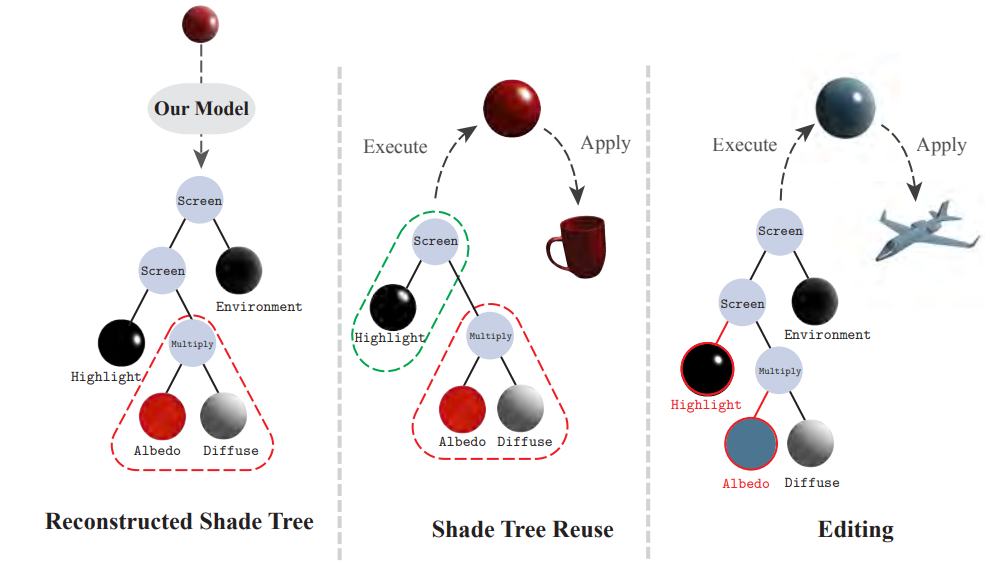
\includegraphics[scale=0.5]{./Imagens/tree-shading.png}
	\end{center}
	\legend{Fonte: \citeonline[p. 24]{lol}}
\end{figure}


Assim como o nosso trabalho, esse artigo se concentra em facilitar o processo para usuários inexperientes, pois ambos visam fornecer ferramentas acessíveis para manipular representações de sombreamento sem exigir conhecimento avançado em programação de shading. Esse artigo também emprega uma representação em árvore, embora para um propósito diferente. Enquanto o nosso trabalho utiliza árvores para representar expressões matemáticas de BRDFs, esse artigo utiliza a decomposição em nós de árvores para representar o shading parcial de objetos.

\subsubsection{A Real-Time Configurable Shader Based on Lookup Tables}



Este trabalho propõe uma arquitetura de hardware que permite cálculos de shading por pixel em tempo real, utilizando lookup-tables. Para isso, são projetados circuitos configurável baseado em lookup-tables, memórias de acesso aleatório (RAMs) e memórias somente leitura (ROMs). Varios circuitos base foram projetados visando realizar cálculos de shading, considerando as operações mais comuns, por exemplo, circuitos para calcular produto interno entre dois vetores, circuitos de rotação de um vetor por um angulo. Ademais, é usado interpolação em um sistema de coordenadas polares em vez da interpolação vetorial convencional com normalização, com o objetivo de reduzir o tamanho dos circuitos e melhorar o desempenho.


\begin{figure}[H]
	\caption{\label{fig_grafico} Exemplo de circuito de produto interno entre vetores}
	\begin{center}
	    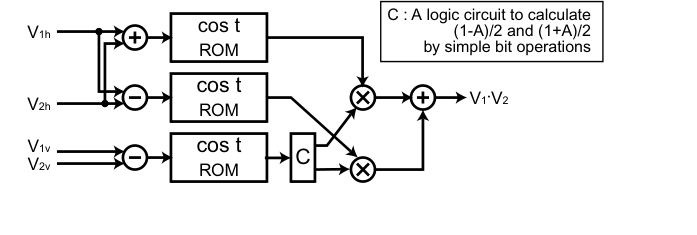
\includegraphics[scale=0.9]{./Imagens/rom-cos-lookup-table.png}
	\end{center}
	\legend{Fonte: \citeonline[p. 24]{lol}}
\end{figure}


Além disso, o circuito suporta diversas BRDFs, como Blinn-Phong, Cook-Torrance, Ward e modelos baseados em microfacetes, com tabelas de lookup específicas para cada modelo. O uso de tabelas de pesquisa permite a representação organizada da parametrização das BRDFs, tornando o processo de transformação de BRDF para shaders mais acessível. Assim como este trabalho, a abordagem facilita a geração de shaders a partir da descrição de BRDFs, apesar da metologia ser diferente.

\section{Pesquisa por Repositórios online}
Também foram analisados repositórios no github e SourceForge, cada um com uma string de busca especifica. Os repositórios encontrados foram filtrados baseados em seus resumos, caso não haja a menção da criação de um compilador, ou não citar uma transformação de BRDF para outra estrutura, esse repositório será excluido.


\begin{table}[H]
\ABNTEXfontereduzida
\caption[bases]{}
\label{tab-bases}
\begin{tabular}{p{2.6cm}|p{6.0cm}|p{2.25cm}|p{3.40cm}}
  %\hline
   \textbf{Plataformas} & \textbf{Termos de Pesquisa}  & \textbf{Resultados}\\
   \hline
   GitHub
   &
   in:readme (GLSL AND BRDF AND  (compiler OR compilation) AND (shader OR shading))
   & 15
   \\ \hline
   SourceForge
   &
   compiler bdrf
   & 0
\end{tabular}
% \legend{Fonte: \citeonline{van86}}
\end{table}


Após ler por completo os resumos dos repostiórios do GitHub, é evidente que nenhum desses projetos é relacionado com o proposto neste trabalhos, apesar de comentar sobre BRDFs, esses projetos não implementam compiladores, não fazem parsing de equações de BRDFs e nem mesmo geram shaders a partir de BRDFs.


\chapter{Conceitos}

\section{BRDFs}

\url{https://www.youtube.com/watch?v=kPIqO929pIc&list=PL2zRqk16wsdpyQNZ6WFlGQtDICpzzQ925&index=3}

\section{Radiometria}

A radiometria trata de conceitos fundamentais relacionados à luz. Ela abrange a capacidade de um material de superfície receber raios de luz de uma direção e refleti-los em outra. No contexto da computação gráfica e renderização, a radiometria desempenha um papel crucial na compreensão do comportamento da luz em uma cena.

A intensidade de um pixel de imagem depende de vários fatores, como iluminação, orientação da superfície e refletância da superfície. A orientação da superfície é determinada pelo vetor normal em um ponto dado, enquanto a refletância da superfície diz respeito às propriedades materiais da mesma.

Para compreender e interpretar a intensidade de um pixel em uma imagem, é essencial compreender os conceitos radiométricos. A radiometria quantifica o brilho de uma fonte de luz, a iluminação de uma superfície, a radiância de uma cena e a refletância da superfície.

Renderização Além da Cor

Renderizar uma imagem envolve mais do que apenas capturar cor. Isso requer conhecimento da intensidade da luz em cada ponto da imagem, isto é, a quantidade de luz incidente na cena que alcança a câmera. A radiometria ajuda na criação de sistemas e unidades para quantificar a radiação eletromagnética, considerando a luz como fótons viajando em linha reta em um modelo óptico geométrico. Esse modelo simplifica considerações de difração e interferência, focando nos caminhos em linha reta dos fótons.

\subsection{Energia Radiante e Fluxo}

Vários processos físicos convertem energia em fótons, como radiação de corpo negro e fusão nuclear em estrelas. Quantificar a energia radiante total envolve entender a energia dos fótons colidindo com um objeto, equivalente ao brilho da imagem. A energia radiante $Q$ considera a energia total de todos os fótons atingindo a cena durante toda a duração.

\begin{align*} 
Q &= \frac{hc}{\lambda} \\
  h &\approx 6,626 \times 10^{-34} J \cdot s (\text{Joules por segundo})\\
  c &\approx 3,00  \times 10^{8} m \cdot s (\text{metros por segundo})\\
  \lambda &\approx 390-700  \times 10^{-3} m (\text{metros})
\end{align*}


É interessante observar a evolução da energia radiante $Q$ ao longo do tempo, isso da origem ao fluxo radiantea $\phi$, medida em impactos de cada fóton por segundo em uma superficie.

\begin{align*} 
  \phi &= \frac{dQ}{dt} [\text{J/s}] 
\end{align*}

A irradiância $E$ quantifica o número de impactos dos photons em uma superficie por segundo por unidade de área. Assim, tempos uma métrica mais específica e essencial para renderizar imagens com precisão.

$$
 E(p) = \frac{d\phi(p)}{dA} [\text{J/s} \cdot m^2]
$$


\subsection{Radiância e BRDF}

A radiância, denotada como $L$, caracteriza a distribuição da luz em um ambiente ao longo de um raio definido por um ponto de origem e uma direção. A radiância desempenha um papel fundamental no cálculo do fluxo por unidade de área em uma superfície considerando toda a luz incidente de todas as direções possiveis em um dado ponto $p$.


\begin{align*} 
  L(p,w) &= \frac{dE_w(p)}{dw} \qquad \left[\frac{J}{s\cdot m^2\cdot \text{sr}}\right]\\ 
E_w &\text{ é função de a irradiancia numa direção $w$ }  \end{align*}


Para acomodar diferentes orientações da superfície e direção do raio, aplicamos o fator $\cos(\theta)$, tal que $\theta$ é o angulo entre a normal da superficie e a direção do $w$ para obter a formula:
\begin{align*} 
  L(p,w) &= \frac{dE(p)}{dw \cos(\theta)} = \frac{d^2\phi(p)}{dAdw \cos(\theta)}
\end{align*}

A radiância pode fornecer informação sobre o quanto um ponto específico está iluminado na direção da câmera. Ela depende não apenas da direção do raio que incide câmera, mas também das propriedades de refletância da superfície. E, no contexto de renderização, a radiância de uma superfície na cena se correlaciona com a irradiância de um pixel em uma imagem da sequinte forma: 

\begin{align*}
  &E(p) = \int_{H^2}{L(p,w)\cos(\theta)dw}\\
  &H^2 \text{ é o hemisfério no plano tangente à superficie no ponto $p$}
\end{align*}


A principal funcionalidade de uma renderizador fotorealista é estimar a radiancia em um ponto $p$ numa dada direção $w_o$. Essa radiancia é dada pela equação de renderização apresentada por @ref Kajiya. Note que essa euquação envolve um termo de radiancia recursiva, o caso base ocorre quando não há mais o termo recursivo, isto é, um fonte de luz na qual sua radiancia é contribuida apenas por randianca emitida $L_e$.

\begin{align*}
  &L_o(p, w_o) = L_e(p, w_o) + 
\int_{H^2}F(p, w_i, w_o){L_i(p,w_i)\cos(\theta)dw_i}\\
    &L_o \text{ é radiancia de saída (\textit{outgoing}) ou {observada}}\\
    &L_e \text{ é radiancia emitida (i.e. fonte de luz)}\\
    &L_i \text{ é radiancia incidente}\\
    &w_i \text{ é a direção incidente}\\
    &w_o \text{ é a direção de saída}\\
    &H^2 \text{ são todas no hemisfério}\\
    &\theta \text{ angulo entre direção incidente e a normal da superficie}\\
    &F \text{ função de refletancia}\\
\end{align*}

A Função de Distribuição Bidirecional de Reflectância (BRDF) descreve como a luz reflete de uma superficie em diferentes direções afetando a radiância de saída. Reflexão é o processo no qual a luz iterage com a superficie sem alterar a sua frequencia. Assim, BRDFs encapsulam as propriedades de reflexão de um material levando em conta vários fatores, como rugosidade da superfície, ângulo de incidência, angulo de reflexão
Formalmente uma BRDF pode ser definida por $F(w_i, w_o)$, onde $w_i$ é a direção indicente de luz e $w_o$ é a direção de saída.

Para BRDFs fisicamente realistas algumas propriedades devem ser respeitadas.

\begin{itemize}
  \item A propriedade de positividade, $ F(\omega_i, \omega_o) \geq 0 $, que garante não existência de energia negativa. 

  \item Também, deve-se obedecer a reciprocidade de Helmhotz, $F(\omega_i, \omega_o) = F(\omega_o, \omega_i)$. Essa reciprocidade é usado na renderização, pois no lugar de traçar os raios da fonte de luz até a camera, podemos traçar os raios da camera até a fonte de luz otimizando a maior parte dos raios traçados diretamente da fonte de luz que não iriam antigir a lente da camera, exitando desperdicio de poder computacional em raios que não contribuem para intensidade de um dado pixel.

  \item A BRDF deve, também, respeitar a conversação de energia, $\forall  \omega_i, \int_{H^2}{F(\omega_i, \omega_o)cos(\theta_o) d\omega_o}\leq 1$. Nesse caso parte da energia pode ser absorvida, ou seja, transformado em outra forma de energia como calor, nesse caso esse somatório infintesimal pode no máximo chegar a 1, mas nunca ultrapassar.
\end{itemize}

\section{BRDF Models}


\subsection{Superfície Pura Especular}
Uma superfície puramente especular reflete a luz apenas em uma direção, seguindo a lei da reflexão. Ela produz reflexões nítidas, semelhantes a espelhos.
A BRDF para uma superfície puramente especular é frequentemente representada pela função delta de Dirac $\delta(\omega_i - \omega_o)$, onde $\omega_i$ é a direção da luz incidente e $\omega_o$ é a direção refletida.
$f(\omega_i, \omega_o) = k_s \cdot \delta(\omega_i - \omega_o)$
A função delta de Dirac garante que toda a luz incidente seja refletida na direção perfeitamente espelhada, resultando em uma reflexão altamente focada e intensa. Esse tipo de superfície é comum em materiais como metal polido ou vidro.

\subsection{BRDF Difusa Ideal}
Uma BRDFs difusa ideal reflete a luz incidente uniformemente em todas as direções, sem preferência por ângulos específicos. é representada por um termo cosseno lambertiano $\frac{\rho_d}{\pi} \cdot \cos \theta$, onde $\rho_d$ é o albedo da superfície e $\theta$ é o ângulo entre a direção da luz incidente e a normal da superfície.
$f(\omega_i, \omega_o) = \frac{\rho_d}{\pi} \cdot \cos \theta$
O termo cosseno garante que a radiância refletida seja proporcional ao cosseno do ângulo entre a direção da luz incidente e a normal da superfície. Esse modelo pode representar superfícies como tinta fosca ou papel.

\subsubsection{BRDF Brilhante (\textit{Glossy})}
Uma superfície brilhante exibe propriedades de reflexão tanto especulares quanto difusas. BRDF para uma superfície brilhante é frequentemente representada por uma combinação de termos especulares e difusos, como o modelo de Blinn-Phong @ref

\subsubsection{BRDF Retro-Refletora}
Uma superfície retro-refletora reflete a luz incidente de volta na direção de onde veio, independentemente do ângulo de incidência. A BRDF para uma superfície retro-refletora envolve tipicamente geometria especializada ou revestimentos projetados para redirecionar a luz de volta para a fonte.

\section{Compiladores}

\subsection{Cadeia de Símbolos e Alfabeto}

Um \textbf{cadeia de símbolos} é uma sequência finita de símbolos retirados de um alfabeto $ \Sigma $. Formalmente, um cadeia $ w $ é representado como $ [w_1, w_2, ..., w_n] $, onde cada $ w_i $ pertence ao alfabeto $ \Sigma $. O \textbf{alfabeto} $ \Sigma $ é um conjunto finito de símbolos distintos usados para construir cadeias em uma linguagem. Ele define os blocos de construção a partir dos quais cadeias válidas na linguagem são formadas.

\subsection{Definições de Linguagens}

Na ciência da computação, as linguagens são sistemas formais compostos por símbolos e regras que são muito uteis para definir um significado algoritimico. Uma \textbf{linguagem} $L$ é definida como um conjunto de cadeias sobre um alfabeto finito $ \Sigma $, $ L \subseteq \Sigma^* $, onde  $ \Sigma^* $ denota o conjunto de todas as cadeias possíveis sobre $ \Sigma $. A estrutura e semântica de uma linguagem  inclue seu alfabeto $ \Sigma $, sintaxe e regras de gramática.

\subsection{Compilador como um Transformação}

Um compilador pode ser visto como um transformação entre linguagens $ L_1 $ e $ L_2 $ que preserva a estrutura interna dos cojuntos, isto é, deve manter o mesmo significado algoritmico. Assim, o compilador $ C: L_1 \rightarrow L_2 $ mapeia programas escritos na linguagem de origem $ L_1 $ para programas equivalentes na linguagem de destino $ L_2 $. Essa transformação garante a preservação semântica, mantendo o comportamento pretendido do programa original durante a tradução.


\section{Gramática}

Para auxiliar na criação de um compilador é necessario entender as regras que auxiliam na validação e geração da linguagem de interesse, esse entedimento pode ser alcaçando pela gramática. Uma gramática $ G $ é um sistema formal composto por um conjunto de regras de produção que especificam como cadeias válidas na linguagem podem ser geradas. Ela inclui terminais, não-terminais, regras de produção e um símbolo inicial.

\begin{itemize}
  \item Terminais: Terminais são os símbolos básicos a partir dos quais as cadeias são formadas. Eles representam as unidades elementares da sintaxe da linguagem.
  \item Não-terminais: Não-terminais são espaços reservados que podem ser substituídos por terminais ou outros não-terminais de acordo com as regras de produção.

  \item Regras de Produção: As regras de produção definem a transformação ou substituição de não-terminais em sequências de terminais e/ou não-terminais.

  \item Símbolo Inicial: O símbolo inicial é um não-terminal especial a partir do qual a derivação de cadeias válidas na linguagem começa.
\end{itemize}


\subsubsection{Gramáticas Livres de Contexto (GLCs)}

Um tipo comum de gramática usado na definição de linguagens é a gramática livre de contexto (GLC). Em uma GLC $ G=(V,\Sigma,R,S)$:

\begin{itemize}
  \item $V$ é um conjunto finito de símbolos não-terminais.

  \item $\Sigma$ é um conjunto finito de símbolos terminais disjunto de $V$.

  \item $R$ é um conjunto finito de regras de produção, cada regra no formato $A \rightarrow \beta$, onde $A$ é um não-terminal e $\beta$ é uma cadeia de terminais e não-terminais.

  \item $S$ é o símbolo inicial, que pertence a $V$.
\end{itemize}

O processo de gerar uma cadeia na linguagem definida por uma gramática é chamado de derivação. Isso envolve aplicar regras de produção sucessivamente, começando pelo símbolo inicial $S$ até restarem apenas símbolos terminais.

Uma árvore sintática é uma representação gráfica do processo de derivação, onde cada nó representa um símbolo na cadeia e cada aresta representa a aplicação de uma regra de produção, nos processos seguintes como análise sintatica,em código, essa árvore é gerada e usada como representação intermediária que auxilia na geração na linguagem alvo $L_2$.


\subsection{Análise Léxica}
A análise léxica, também conhecida como \textit{lexing} ou \textit{tokenization}, é a primeira etapa do processo de compilação, na qual a entrada textual é dividida em unidades léxicas significativas chamadas de \textit{tokens}. Esses tokens representam os componentes básicos da linguagem, como palavras-chave, identificadores, operadores e literais. O analisador léxico percorre o código fonte caractere por caractere, agrupando-os em tokens conforme regras pré-definidas pela gramática da linguagem.

\subsection{Análise Sintática ou \textit{Parsing}}
A análise sintática é a segunda fase do processo de compilação, na qual os tokens gerados pela análise léxica são organizados e verificados quanto à conformidade com a gramática da linguagem. Essa etapa envolve a construção de uma árvore sintática ou estrutura de dados equivalente que representa a estrutura hierárquica das expressões e instruções do programa. O analisador sintático utiliza regras de produção gramatical para validar a sintaxe do código fonte e identificar possíveis erros.

\subsection{Pratt Parsing}
O Pratt Parsing, introduzida por Vaughan Pratt, é uma técnica de análise sintática recursiva que permite analisar expressões com precedência de operadores de forma eficiente e sem ambiguidades. Uma das características distintivas do Pratt Parsing é a maneira como lida com a precedência dos operadores, que é determinada pela ordem de avaliação das expressões. Ao contrário da análise descendente recursiva tradicional, onde cada não-terminal possui uma função de análise, a análise Pratt associa funções de manipulação (handlers) com tokens. Essas funções de manipulação são responsáveis por analisar expressões envolvendo seus respectivos tokens.

\subsubsection{Precedência de Expressões}

Na implementação do Pratt Parser, a precedência das expressões é definida por meio de uma tabela de precedência, na qual cada operador é associado a um nível de precedência. Isso permite que o parser decida dinamicamente a ordem de avaliação das expressões com base nos operadores encontrados durante a análise.

Essa abordagem simplifica significativamente a implementação do parser e elimina a necessidade de criar uma grammática que encapsula a precendencia em sua definição, também evita recursão profunda para lidar com diferentes níveis de precedência, tornando o Pratt Parsing uma técnica eficiente para análise sintática.

\subsubsection{Árvores mais à Direita e mais à Esquerda}

Na análise Pratt, a estrutura da árvore de expressão pode ser influenciada pela ordem de avaliação dos operadores. Essa distinção leva a dois tipos principais de árvores de expressão: árvores inclinadas à direita e árvores inclinadas à esquerda.

\textbf{Árvore inclinada à Direita:} Em uma árvore inclinada à direita, operadores com maior precedência são resolvidos primeiro, mesmo que apareçam mais tarde (para a direita) na expressão. Isso resulta em uma árvore onde os operadores com maior precedência estão mais próximos da raiz, indicando que eles são avaliados primeiro. Considere a expressão `1 + 2 * 3`. Apesar de `*` aparecer após `+`, ele tem uma precedência mais alta e, portanto, forma uma subárvore que é resolvida antes da adição. A árvore resultante é:


\begin{verbatim}
               +
              / \
             1   *
                / \
               2   3
\end{verbatim}

\textbf{Árvore inclinada à Esquerda:} Por outro lado, em uma árvore inclinada à esquerda, operadores com maior precedência são resolvidos por último, seguindo uma ordem de avaliação da esquerda para a direita. Isso significa que operadores com maior precedência formam subárvores que são resolvidas mais profundamente na árvore. As árvores inclinadas à esquerda estão tipicamente associadas a chamadas recursivas na análise.

Para alcançar a estrutura desejada da árvore, o Pratt parsing utiliza as estratégias de recursão e iteração com base na precedência dos operadores para saber o momento de gerar uma subarvores inclinada para esquerda ou direita. Operadores com precedência maior que a do operador atual formam a estrutura inclinada à direita, enquanto operadores com precedência menor formam a estrutura inclinada à esquerda.

\subsubsection{Pseudo-código para Análise de Expressões}

O pseudo-código \ref{alg1},
demonstra o Pratt \textit{parsing} para a construção de árvores de expressão, considerando tanto estruturas inclinadas à direita quanto à esquerda. Esse algoritmo também é robusto mesmo quando um operador é tanto infixo quanto prefixo, por exemplo "$-$" pode ser um \textit{token} de subtração ou de negação. Assim cada token tem uma função de prefixo e infixo associada.

Nesse algoritimo, 
\textbf{proximo\_token()} recupera o próximo elemento da lista de tokens,
\textbf{token.precedencia}() retorna a precedencia do token atual, \textbf{token.prefixo()} é a função associada ao token que realisa o parsing de uma expressão quando o token é o primeiro em uma subexpressão (e.g. o token "$-$" é o primeiro na expressão "$-3$"). Já o   
\textbf{token.infixo}(esquerda) é a função associada ao token uma função que cria um nó subárvore utilizando outra subarvore já criada como entrada para gerar expressão com operadores infixos, por exemplo a subarvore esquerda pode ser a expressão "$-3$", o token atual ser "$*$" e o o retorno gera a expressão completa "$-3 * 1$"

Tanto \textbf{token.infixo} quanto \textbf{token.prefixo} podem ser indiretamente recursivas, isto é, ambas podem chamar a função \textbf{expressao} no algortimo \ref{alg1}. 
Por fim, \textbf{precedencia\_anterior} representa a precedência do token anterior, garantindo que os operadores sejam resolvidos na ordem correta.

\begin{algoritmo}[H]
	\caption{Função Pratt Parsing de Expressão}
	\label{alg1}
	\label{alg1}
  \begin{lstlisting}
  function expressao(precedencia_anterior:=0):
      token := proximo_token()
      esquerda := token.prefixo()
      while precedencia_anterior < token.precedencia():
          token    = proximo_token()
          esquerda = token.infixo(esquerda)
      return esquerda
  \end{lstlisting}
\end{algoritmo}

% \begin{verbatim}
% def expressao(precedencia_anterior:=0):
%     token = proximo_token()
%     esquerda = token.prefixo()  # denotação nula
%
%     while precedencia_anterior < token.precedencia():
%         token = proximo_token()
%         esquerda = token.infixo(esquerda)  # denotação à esquerda
%
%     return esquerda
% \end{verbatim}

% Neste pseudo-código:
% - `proximo_token()` recupera o próximo token do fluxo de tokens.
% - `token.prefixo()` é uma função associada ao token que analisa a expressão quando o token é o primeiro token em uma subexpressão.
% - `token.infixo(esquerda)` é uma função associada ao token que analisa a expressão quando o token não é o primeiro token em uma subexpressão, recebendo o operando esquerdo como entrada.
% - `precedencia_anterior` representa a precedência do token anterior, garantindo que os operadores sejam resolvidos na ordem correta com base na precedência.


\section{Geração da Linguagem Alvo}
\section{\textit{Shaders}}
\subsection{Fragment}
\subsection{Fragment}


% \chapter{Resultados de comandos}\label{cap_exemplos}

\chapterprecis{Isto é uma sinopse de capítulo. A ABNT não traz nenhuma
normatização a respeito desse tipo de resumo, que é mais comum em romances 
e livros técnicos.}\index{sinopse de capítulo}

% ---
\section{Codificação dos arquivos: UTF8}
% ---

A codificação de todos os arquivos do \abnTeX\ é \texttt{UTF8}. É necessário que
você utilize a mesma codificação nos documentos que escrever, inclusive nos
arquivos de base bibliográficas |.bib|.

% ---
\section{Citações diretas}
\label{sec-citacao}
% ---

\index{citações!diretas}Utilize o ambiente \texttt{citacao} para incluir citações diretas com mais de três linhas:

\begin{citacao}
As citações diretas, no texto, com mais de três linhas, devem ser
destacadas com recuo de 4 cm da margem esquerda, com letra menor que a do texto utilizado e sem as aspas. No caso de documentos datilografados, deve-se observar apenas o recuo \cite[5.3]{NBR10520:2002}.
\end{citacao}

Use o ambiente assim:

\begin{verbatim}
\begin{citacao}
As citações diretas, no texto, com mais de três linhas [...] 
deve-se observar apenas o recuo \cite[5.3]{NBR10520:2002}.
\end{citacao}
\end{verbatim}

O ambiente \texttt{citacao} pode receber como parâmetro opcional um nome de
idioma previamente carregado nas opções da classe (\autoref{sec-hifenizacao}). Nesse
caso, o texto da citação é automaticamente escrito em itálico e a hifenização é
ajustada para o idioma selecionado na opção do ambiente. Por exemplo:

\begin{verbatim}
\begin{citacao}[english]
Text in English language in italic with correct hyphenation.
\end{citacao}
\end{verbatim}

Tem como resultado:

\begin{citacao}[english]
Text in English language in italic with correct hyphenation.
\end{citacao}

\index{citações!simples}Citações simples, com até três linhas, devem ser
incluídas com aspas. Observe que em \LaTeX as aspas iniciais são diferentes das
finais: ``Amor é fogo que arde sem se ver''.

% ---
\section{Notas de rodapé}
% ---

As notas de rodapé são detalhadas pela NBR 14724:2011 na seção 5.2.1\footnote{As
notas devem ser digitadas ou datilografadas dentro das margens, ficando
separadas do texto por um espaço simples de entre as linhas e por filete de 5
cm, a partir da margem esquerda. Devem ser alinhadas, a partir da segunda linha
da mesma nota, abaixo da primeira letra da primeira palavra, de forma a destacar
o expoente, sem espaço entre elas e com fonte menor
\citeonline[5.2.1]{NBR14724:2011}.}\footnote{Caso uma série de notas sejam
criadas sequencialmente, o \abnTeX\ instrui o \LaTeX\ para que uma vírgula seja
colocada após cada número do expoente que indica a nota de rodapé no corpo do
texto.}\footnote{Verifique se os números do expoente possuem uma vírgula para
dividi-los no corpo do texto.}. 


% ---
\section{Tabelas}
% ---

\index{tabelas}A \autoref{tab-nivinv} é um exemplo de tabela construída em
\LaTeX.

\begin{table}[htb]
\ABNTEXfontereduzida
\caption[Níveis de investigação]{Níveis de investigação.}
\label{tab-nivinv}
\begin{tabular}{p{2.6cm}|p{6.0cm}|p{2.25cm}|p{3.40cm}}
  %\hline
   \textbf{Nível de Investigação} & \textbf{Insumos}  & \textbf{Sistemas de Investigação}  & \textbf{Produtos}  \\
    \hline
    Meta-nível & Filosofia\index{filosofia} da Ciência  & Epistemologia &
    Paradigma  \\
    \hline
    Nível do objeto & Paradigmas do metanível e evidências do nível inferior &
    Ciência  & Teorias e modelos \\
    \hline
    Nível inferior & Modelos e métodos do nível do objeto e problemas do nível inferior & Prática & Solução de problemas  \\
   % \hline
\end{tabular}
\legend{Fonte: \citeonline{van86}}
\end{table}

Já a \autoref{tabela-ibge} apresenta uma tabela criada conforme o padrão do
\citeonline{ibge1993} requerido pelas normas da ABNT para documentos técnicos e
acadêmicos.

\begin{table}[htb]
\IBGEtab{%
  \caption{Um Exemplo de tabela alinhada que pode ser longa
  ou curta, conforme padrão IBGE.}%
  \label{tabela-ibge}
}{%
  \begin{tabular}{ccc}
  \toprule
   Nome & Nascimento & Documento \\
  \midrule \midrule
   Maria da Silva & 11/11/1111 & 111.111.111-11 \\
  \midrule 
   João Souza & 11/11/2111 & 211.111.111-11 \\
  \midrule 
   Laura Vicuña & 05/04/1891 & 3111.111.111-11 \\
  \bottomrule
\end{tabular}%
}{%
  \fonte{Produzido pelos autores.}%
  \nota{Esta é uma nota, que diz que os dados são baseados na
  regressão linear.}%
  \nota[Anotações]{Uma anotação adicional, que pode ser seguida de várias
  outras.}%
  }
\end{table}


% ---
\section{Figuras}
% ---

\index{figuras}Figuras podem ser criadas diretamente em \LaTeX,
como o exemplo da \autoref{fig_circulo}.

\begin{figure}[htb]
	\caption{\label{fig_circulo}A delimitação do espaço}
	\begin{center}
	    \setlength{\unitlength}{5cm}
		\begin{picture}(1,1)
		\put(0,0){\line(0,1){1}}
		\put(0,0){\line(1,0){1}}
		\put(0,0){\line(1,1){1}}
		\put(0,0){\line(1,2){.5}}
		\put(0,0){\line(1,3){.3333}}
		\put(0,0){\line(1,4){.25}}
		\put(0,0){\line(1,5){.2}}
		\put(0,0){\line(1,6){.1667}}
		\put(0,0){\line(2,1){1}}
		\put(0,0){\line(2,3){.6667}}
		\put(0,0){\line(2,5){.4}}
		\put(0,0){\line(3,1){1}}
		\put(0,0){\line(3,2){1}}
		\put(0,0){\line(3,4){.75}}
		\put(0,0){\line(3,5){.6}}
		\put(0,0){\line(4,1){1}}
		\put(0,0){\line(4,3){1}}
		\put(0,0){\line(4,5){.8}}
		\put(0,0){\line(5,1){1}}
		\put(0,0){\line(5,2){1}}
		\put(0,0){\line(5,3){1}}
		\put(0,0){\line(5,4){1}}
		\put(0,0){\line(5,6){.8333}}
		\put(0,0){\line(6,1){1}}
		\put(0,0){\line(6,5){1}}
		\end{picture}
	\end{center}
	\legend{Fonte: os autores}
\end{figure}

Ou então figuras podem ser incorporadas de arquivos externos, como é o caso da
\autoref{fig_grafico}. Se a figura que for incluída se tratar de um diagrama, um
gráfico ou uma ilustração que você mesmo produza, priorize o uso de imagens
vetoriais no formato PDF. Com isso, o tamanho do arquivo final do trabalho será
menor, e as imagens terão uma apresentação melhor, principalmente quando
impressas, uma vez que imagens vetorias são perfeitamente escaláveis para
qualquer dimensão. Nesse caso, se for utilizar o Microsoft Excel para produzir
gráficos, ou o Microsoft Word para produzir ilustrações, exporte-os como PDF e
os incorpore ao documento conforme o exemplo abaixo. No entanto, para manter a
coerência no uso de software livre (já que você está usando \LaTeX e \abnTeX),
teste a ferramenta \textsf{InkScape}\index{InkScape}
(\url{http://inkscape.org/}). Ela é uma excelente opção de código-livre para
produzir ilustrações vetoriais, similar ao CorelDraw\index{CorelDraw} ou ao Adobe
Illustrator\index{Adobe Illustrator}. De todo modo, caso não seja possível
utilizar arquivos de imagens como PDF, utilize qualquer outro formato, como
JPEG, GIF, BMP, etc. Nesse caso, você pode tentar aprimorar as imagens
incorporadas com o software livre \textsf{Gimp}\index{Gimp}
(\url{http://www.gimp.org/}). Ele é uma alternativa livre ao Adobe
Photoshop\index{Adobe Photoshop}.

\begin{figure}[htb]
	\caption{\label{fig_grafico}Gráfico produzido em Excel e salvo como PDF}
	\begin{center}
	    \includegraphics[scale=0.5]{Imagens/abntex2-modelo-img-marca.pdf}
	\end{center}
	\legend{Fonte: \citeonline[p. 24]{araujo2012}}
\end{figure}

% ---
\subsection{Figuras em \emph{minipages}}
% ---

\emph{Minipages} são usadas para inserir textos ou outros elementos em quadros
com tamanhos e posições controladas. Veja o exemplo da
\autoref{fig_minipage_imagem1} e da \autoref{fig_minipage_grafico2}.

\begin{figure}[htb]
 \label{teste}
 \centering
  \begin{minipage}{0.4\textwidth}
    \centering
    \caption{Imagem 1 da minipage} \label{fig_minipage_imagem1}
    \includegraphics[scale=0.9]{Imagens/abntex2-modelo-img-marca.pdf}
    \legend{Fonte: Produzido pelos autores}
  \end{minipage}
  \hfill
  \begin{minipage}{0.4\textwidth}
    \centering
    \caption{Grafico 2 da minipage} \label{fig_minipage_grafico2}
    \includegraphics[scale=0.2]{Imagens/abntex2-modelo-img-grafico.pdf}
    \legend{Fonte: \citeonline[p. 24]{araujo2012}}
  \end{minipage}
\end{figure}

Observe que, segundo a \citeonline[seções 4.2.1.10 e 5.8]{NBR14724:2011}, as
ilustrações devem sempre ter numeração contínua e única em todo o documento:

\begin{citacao}
Qualquer que seja o tipo de ilustração, sua identificação aparece na parte
superior, precedida da palavra designativa (desenho, esquema, fluxograma,
fotografia, gráfico, mapa, organograma, planta, quadro, retrato, figura,
imagem, entre outros), seguida de seu número de ordem de ocorrência no texto,
em algarismos arábicos, travessão e do respectivo título. Após a ilustração, na
parte inferior, indicar a fonte consultada (elemento obrigatório, mesmo que
seja produção do próprio autor), legenda, notas e outras informações
necessárias à sua compreensão (se houver). A ilustração deve ser citada no
texto e inserida o mais próximo possível do trecho a que se
refere. \cite[seções 5.8]{NBR14724:2011}
\end{citacao}

% ---
\section{Expressões matemáticas}
% ---

\index{expressões matemáticas}Use o ambiente \texttt{equation} para escrever
expressões matemáticas numeradas:

\begin{equation}
  \forall x \in X, \quad \exists \: y \leq \epsilon
\end{equation}

Escreva expressões matemáticas entre \$ e \$, como em $ \lim_{x \to \infty}
\exp(-x) = 0 $, para que fiquem na mesma linha.

Também é possível usar colchetes para indicar o início de uma expressão
matemática que não é numerada.

\[
\left|\sum_{i=1}^n a_ib_i\right|
\le
\left(\sum_{i=1}^n a_i^2\right)^{1/2}
\left(\sum_{i=1}^n b_i^2\right)^{1/2}
\]

Consulte mais informações sobre expressões matemáticas em
\url{https://github.com/abntex/abntex2/wiki/Referencias}.

% ---
\section{Enumerações: alíneas e subalíneas}
% ---

\index{alíneas}\index{subalíneas}\index{incisos}Quando for necessário enumerar
os diversos assuntos de uma seção que não possua título, esta deve ser
subdividida em alíneas \cite[4.2]{NBR6024:2012}:

\begin{alineas}

  \item os diversos assuntos que não possuam título próprio, dentro de uma mesma
  seção, devem ser subdivididos em alíneas; 
  
  \item o texto que antecede as alíneas termina em dois pontos;
  \item as alíneas devem ser indicadas alfabeticamente, em letra minúscula,
  seguida de parêntese. Utilizam-se letras dobradas, quando esgotadas as
  letras do alfabeto;

  \item as letras indicativas das alíneas devem apresentar recuo em relação à
  margem esquerda;

  \item o texto da alínea deve começar por letra minúscula e terminar em
  ponto-e-vírgula, exceto a última alínea que termina em ponto final;

  \item o texto da alínea deve terminar em dois pontos, se houver subalínea;

  \item a segunda e as seguintes linhas do texto da alínea começa sob a
  primeira letra do texto da própria alínea;
  
  \item subalíneas \cite[4.3]{NBR6024:2012} devem ser conforme as alíneas a
  seguir:

  \begin{alineas}
     \item as subalíneas devem começar por travessão seguido de espaço;

     \item as subalíneas devem apresentar recuo em relação à alínea;

     \item o texto da subalínea deve começar por letra minúscula e terminar em
     ponto-e-vírgula. A última subalínea deve terminar em ponto final, se não
     houver alínea subsequente;

     \item a segunda e as seguintes linhas do texto da subalínea começam sob a
     primeira letra do texto da própria subalínea.
  \end{alineas}
  
  \item no \abnTeX\ estão disponíveis os ambientes \texttt{incisos} e
  \texttt{subalineas}, que em suma são o mesmo que se criar outro nível de
  \texttt{alineas}, como nos exemplos à seguir:
  
  \begin{incisos}
    \item \textit{Um novo inciso em itálico};
  \end{incisos}
  
  \item Alínea em \textbf{negrito}:
  
  \begin{subalineas}
    \item \textit{Uma subalínea em itálico};
    \item \underline{\textit{Uma subalínea em itálico e sublinhado}}; 
  \end{subalineas}
  
  \item Última alínea com \emph{ênfase}.
  
\end{alineas}

% ---
\section{Espaçamento entre parágrafos e linhas}
% ---

\index{espaçamento!dos parágrafos}O tamanho do parágrafo, espaço entre a margem
e o início da frase do parágrafo, é definido por:

\begin{verbatim}
   \setlength{\parindent}{1.3cm}
\end{verbatim}

\index{espaçamento!do primeiro parágrafo}Por padrão, não há espaçamento no
primeiro parágrafo de cada início de divisão do documento
(\autoref{sec-divisoes}). Porém, você pode definir que o primeiro parágrafo
também seja indentado, como é o caso deste documento. Para isso, apenas inclua o
pacote \textsf{indentfirst} no preâmbulo do documento:

\begin{verbatim}
   \usepackage{indentfirst}      % Indenta o primeiro parágrafo de cada seção.
\end{verbatim}

\index{espaçamento!entre os parágrafos}O espaçamento entre um parágrafo e outro
pode ser controlado por meio do comando:

\begin{verbatim}
  \setlength{\parskip}{0.2cm}  % tente também \onelineskip
\end{verbatim}

\index{espaçamento!entre as linhas}O controle do espaçamento entre linhas é
definido por:

\begin{verbatim}
  \OnehalfSpacing       % espaçamento um e meio (padrão); 
  \DoubleSpacing        % espaçamento duplo
  \SingleSpacing        % espaçamento simples	
\end{verbatim}

Para isso, também estão disponíveis os ambientes:

\begin{verbatim}
  \begin{SingleSpace} ...\end{SingleSpace}
  \begin{Spacing}{hfactori} ... \end{Spacing}
  \begin{OnehalfSpace} ... \end{OnehalfSpace}
  \begin{OnehalfSpace*} ... \end{OnehalfSpace*}
  \begin{DoubleSpace} ... \end{DoubleSpace}
  \begin{DoubleSpace*} ... \end{DoubleSpace*} 
\end{verbatim}

Para mais informações, consulte \citeonline[p. 47-52 e 135]{memoir}.

% ---
\section{Inclusão de outros arquivos}\label{sec-include}
% ---

É uma boa prática dividir o seu documento em diversos arquivos, e não
apenas escrever tudo em um único. Esse recurso foi utilizado neste
documento. Para incluir diferentes arquivos em um arquivo principal,
de modo que cada arquivo incluído fique em uma página diferente, utilize o
comando:

\begin{verbatim}
   \include{documento-a-ser-incluido}      % sem a extensão .tex
\end{verbatim}

Para incluir documentos sem quebra de páginas, utilize:

\begin{verbatim}
   \input{documento-a-ser-incluido}      % sem a extensão .tex
\end{verbatim}

% ---
\section{Compilar o documento \LaTeX}
% ---

Geralmente os editores \LaTeX, como o
TeXlipse\footnote{\url{http://texlipse.sourceforge.net/}}, o
Texmaker\footnote{\url{http://www.xm1math.net/texmaker/}}, entre outros,
compilam os documentos automaticamente, de modo que você não precisa se
preocupar com isso.

No entanto, você pode compilar os documentos \LaTeX usando os seguintes
comandos, que devem ser digitados no \emph{Prompt de Comandos} do Windows ou no
\emph{Terminal} do Mac ou do Linux:

\begin{verbatim}
   pdflatex ARQUIVO_PRINCIPAL.tex
   bibtex ARQUIVO_PRINCIPAL.aux
   makeindex ARQUIVO_PRINCIPAL.idx 
   makeindex ARQUIVO_PRINCIPAL.nlo -s nomencl.ist -o ARQUIVO_PRINCIPAL.nls
   pdflatex ARQUIVO_PRINCIPAL.tex
   pdflatex ARQUIVO_PRINCIPAL.tex
\end{verbatim}

% ---
\section{Remissões internas}
% ---

Ao nomear a \autoref{tab-nivinv} e a \autoref{fig_circulo}, apresentamos um
exemplo de remissão interna, que também pode ser feita quando indicamos o
\autoref{cap_exemplos}, que tem o nome \emph{\nameref{cap_exemplos}}. O número
do capítulo indicado é \ref{cap_exemplos}, que se inicia à
\autopageref{cap_exemplos}\footnote{O número da página de uma remissão pode ser
obtida também assim:
\pageref{cap_exemplos}.}.
Veja a \autoref{sec-divisoes} para outros exemplos de remissões internas entre
seções, subseções e subsubseções.

O código usado para produzir o texto desta seção é:

\begin{verbatim}
Ao nomear a \autoref{tab-nivinv} e a \autoref{fig_circulo}, apresentamos um
exemplo de remissão interna, que também pode ser feita quando indicamos o
\autoref{cap_exemplos}, que tem o nome \emph{\nameref{cap_exemplos}}. O número
do capítulo indicado é \ref{cap_exemplos}, que se inicia à
\autopageref{cap_exemplos}\footnote{O número da página de uma remissão pode ser
obtida também assim:
\pageref{cap_exemplos}.}.
Veja a \autoref{sec-divisoes} para outros exemplos de remissões internas entre
seções, subseções e subsubseções.
\end{verbatim}

% ---
\section{Divisões do documento: seção}\label{sec-divisoes}
% ---

Esta seção testa o uso de divisões de documentos. Esta é a
\autoref{sec-divisoes}. Veja a \autoref{sec-divisoes-subsection}.

\subsection{Divisões do documento: subseção}\label{sec-divisoes-subsection}

Isto é uma subseção. Veja a \autoref{sec-divisoes-subsubsection}, que é uma
\texttt{subsubsection} do \LaTeX, mas é impressa chamada de ``subseção'' porque
no Português não temos a palavra ``subsubseção''.

\subsubsection{Divisões do documento: subsubseção}
\label{sec-divisoes-subsubsection}

Isto é uma subsubseção.

\subsubsection{Divisões do documento: subsubseção}

Isto é outra subsubseção.

\subsection{Divisões do documento: subseção}\label{sec-exemplo-subsec}

Isto é uma subseção.

\subsubsection{Divisões do documento: subsubseção}

Isto é mais uma subsubseção da \autoref{sec-exemplo-subsec}.


\subsubsubsection{Esta é uma subseção de quinto
nível}\label{sec-exemplo-subsubsubsection}

Esta é uma seção de quinto nível. Ela é produzida com o seguinte comando:

\begin{verbatim}
\subsubsubsection{Esta é uma subseção de quinto
nível}\label{sec-exemplo-subsubsubsection}
\end{verbatim}

\subsubsubsection{Esta é outra subseção de quinto nível}\label{sec-exemplo-subsubsubsection-outro}

Esta é outra seção de quinto nível.


\paragraph{Este é um parágrafo numerado}\label{sec-exemplo-paragrafo}

Este é um exemplo de parágrafo nomeado. Ele é produzida com o comando de
parágrafo:

\begin{verbatim}
\paragraph{Este é um parágrafo nomeado}\label{sec-exemplo-paragrafo}
\end{verbatim}

A numeração entre parágrafos numeradaos e subsubsubseções são contínuas.

\paragraph{Esta é outro parágrafo numerado}\label{sec-exemplo-paragrafo-outro}

Esta é outro parágrafo nomeado.

% ---
\section{Este é um exemplo de nome de seção longo. Ele deve estar
alinhado à esquerda e a segunda e demais linhas devem iniciar logo abaixo da
primeira palavra da primeira linha}
% ---

Isso atende à norma \citeonline[seções de 5.2.2 a 5.2.4]{NBR14724:2011} 
 e \citeonline[seções de 3.1 a 3.8]{NBR6024:2012}.

% ---
\section{Diferentes idiomas e hifenizações}
\label{sec-hifenizacao}
% ---

Para usar hifenizações de diferentes idiomas, inclua nas opções do documento o
nome dos idiomas que o seu texto contém. Por exemplo (para melhor
visualização, as opções foram quebras em diferentes linhas):

\begin{verbatim}
\documentclass[
	12pt,
	openright,
	twoside,
	a4paper,
	english,
	french,
	spanish,
	brazil
	]{abntex2}
\end{verbatim}

O idioma português-brasileiro (\texttt{brazil}) é incluído automaticamente pela
classe \textsf{abntex2}. Porém, mesmo assim a opção \texttt{brazil} deve ser
informada como a última opção da classe para que todos os pacotes reconheçam o
idioma. Vale ressaltar que a última opção de idioma é a utilizada por padrão no
documento. Desse modo, caso deseje escrever um texto em inglês que tenha
citações em português e em francês, você deveria usar o preâmbulo como abaixo:

\begin{verbatim}
\documentclass[
	12pt,
	openright,
	twoside,
	a4paper,
	french,
	brazil,
	english
	]{abntex2}
\end{verbatim}

A lista completa de idiomas suportados, bem como outras opções de hifenização,
estão disponíveis em \citeonline[p.~5-6]{babel}.

Exemplo de hifenização em inglês\footnote{Extraído de:
\url{http://en.wikibooks.org/wiki/LaTeX/Internationalization}}:

\begin{otherlanguage*}{english}
\textit{Text in English language. This environment switches all language-related
definitions, like the language specific names for figures, tables etc. to the other
language. The starred version of this environment typesets the main text
according to the rules of the other language, but keeps the language specific
string for ancillary things like figures, in the main language of the document.
The environment hyphenrules switches only the hyphenation patterns used; it can
also be used to disallow hyphenation by using the language name
`nohyphenation'.}
\end{otherlanguage*}

O idioma geral do texto por ser alterado como no exemplo seguinte:

\begin{verbatim}
  \selectlanguage{english}
\end{verbatim}

Isso altera automaticamente a hifenização e todos os nomes constantes de
referências do documento para o idioma inglês. Consulte o manual da classe
\cite{abntex2classe} para obter orientações adicionais sobre internacionalização de
documentos produzidos com \abnTeX.

A \autoref{sec-citacao} descreve o ambiente \texttt{citacao} que pode receber
como parâmetro um idioma a ser usado na citação.

% ---
\section{Consulte o manual da classe \textsf{abntex2}}
% ---

Consulte o manual da classe \textsf{abntex2} \cite{abntex2classe} para uma
referência completa das macros e ambientes disponíveis. 

Além disso, o manual possui informações adicionais sobre as normas ABNT
observadas pelo \abnTeX\ e considerações sobre eventuais requisitos específicos
não atendidos, como o caso da \citeonline[seção 5.2.2]{NBR14724:2011}, que
especifica o espaçamento entre os capítulos e o início do texto, regra
propositalmente não atendida pelo presente modelo.

% ---
\section{Referências bibliográficas}
% ---

A formatação das referências bibliográficas conforme as regras da ABNT são um
dos principais objetivos do \abnTeX. Consulte os manuais
\citeonline{abntex2cite} e \citeonline{abntex2cite-alf} para obter informações
sobre como utilizar as referências bibliográficas.

%-
\subsection{Acentuação de referências bibliográficas}
%-

Normalmente não há problemas em usar caracteres acentuados em arquivos
bibliográficos (\texttt{*.bib}). Porém, como as regras da ABNT fazem uso quase
abusivo da conversão para letras maiúsculas, é preciso observar o modo como se
escreve os nomes dos autores. Na ~\autoref{tabela-acentos} você encontra alguns
exemplos das conversões mais importantes. Preste atenção especial para `ç' e `í'
que devem estar envoltos em chaves. A regra geral é sempre usar a acentuação
neste modo quando houver conversão para letras maiúsculas.

\begin{table}[htbp]
\caption{Tabela de conversão de acentuação.}
\label{tabela-acentos}

\begin{center}
\begin{tabular}{ll}\hline\hline
acento & \textsf{bibtex}\\
à á ã & \verb+\`a+ \verb+\'a+ \verb+\~a+\\
í & \verb+{\'\i}+\\
ç & \verb+{\c c}+\\
\hline\hline
\end{tabular}
\end{center}
\end{table}


% ---
\section{Precisa de ajuda?}
% ---

Consulte a FAQ com perguntas frequentes e comuns no portal do \abnTeX:
\url{https://github.com/abntex/abntex2/wiki/FAQ}.

Inscreva-se no grupo de usuários \LaTeX:
\url{http://groups.google.com/group/latex-br}, tire suas dúvidas e ajude
outros usuários.

Participe também do grupo de desenvolvedores do \abnTeX:
\url{http://groups.google.com/group/abntex2} e faça sua contribuição à
ferramenta.

% ---
\section{Você pode ajudar?}
% ---

Sua contribuição é muito importante! Você pode ajudar na divulgação, no
desenvolvimento e de várias outras formas. Veja como contribuir com o \abnTeX\
em \url{https://github.com/abntex/abntex2/wiki/Como-Contribuir}.

% ---
\section{Quer customizar os modelos do \abnTeX\ para sua instituição ou universidade?}
% ---

Veja como customizar o \abnTeX\ em: \\
\url{https://github.com/abntex/abntex2/wiki/ComoCustomizar}.

% \chapter{Conteúdos específicos do modelo de trabalho acadêmico}\label{cap_trabalho_academico}

\section{Quadros}

Este modelo vem com o ambiente \texttt{quadro} e impressão de Lista de quadros 
configurados por padrão. Verifique um exemplo de utilização:

\begin{quadro}[htb]
\caption{\label{quadro_exemplo}Exemplo de quadro}
\begin{tabular}{|c|c|c|c|}
	\hline
	\textbf{Pessoa} & \textbf{Idade} & \textbf{Peso} & \textbf{Altura} \\ \hline
	Marcos & 26    & 68   & 178    \\ \hline
	Ivone  & 22    & 57   & 162    \\ \hline
	...    & ...   & ...  & ...    \\ \hline
	Sueli  & 40    & 65   & 153    \\ \hline
\end{tabular}
\fonte{Autor.}
\end{quadro}

Este parágrafo apresenta como referenciar o quadro no texto, requisito
obrigatório da ABNT. 
Primeira opção, utilizando \texttt{autoref}: Ver o \autoref{quadro_exemplo}. 
Segunda opção, utilizando  \texttt{ref}: Ver o Quadro \ref{quadro_exemplo}.

% % ---
% Capitulo de revisão de literatura
% ---
\chapter{Lorem ipsum dolor sit amet}
% ---

% ---
\section{Aliquam vestibulum fringilla lorem}
% ---

\lipsum[1]

\lipsum[2-3]

% ---
% primeiro capitulo de Resultados
% ---
\chapter{Lectus lobortis condimentum}
% ---

% ---
\section{Vestibulum ante ipsum primis in faucibus orci luctus et ultrices
posuere cubilia Curae}
% ---

\lipsum[21-22]

% ---
% segundo capitulo de Resultados
% ---
\chapter{Nam sed tellus sit amet lectus urna ullamcorper tristique interdum
elementum}
% ---

% ---
\section{Pellentesque sit amet pede ac sem eleifend consectetuer}
% ---

\lipsum[24]
% \chapter{Customização DCOMP}

\section{Lista de códigos}

Usado para criar a lista de códigos, adicionar sintaxe highlight, enumerar as linhas e colorir o fundo, para dar destaque a implementação.

Sintaxe básica:
\begin{verbatim}
\begin{codigo}[!htb]
    \caption{Espaço para o título do código}
    \label{Espaço para o label do código, para ser usado na referência}  
    \begin{lstlisting}[language = Linguagem de programação a ser usada]
        <CÓDIGO>
    \end{lstlisting}
\end{codigo}
\end{verbatim}

\begin{codigo}[htb]
  \caption{Código PHP}
  \label{codigophp}
  \begin{lstlisting}[language = php]
       <?php

       echo '%*Olá mundo*)!';
       print '%*Olá mundo*)!';
  \end{lstlisting}
\end{codigo}

\begin{codigo}
  \caption{Código python}
  \label{codigopython}
  \begin{lstlisting}[language = python]
    import numpy as np
 
    def incmatrix(genl1, genl2):
        m = len(genl1)
        n = len(genl2)
        M = None #to become the incidence matrix
        VT = np.zeros((n*m,1), int)  #dummy variable
 
        #compute the bitwise xor matrix
        M1 = bitxormatrix(genl1)
        M2 = np.triu(bitxormatrix(genl2),1) 
 
        for i in range(m-1):
            for j in range(i+1, m):
                [r,c] = np.where(M2 == M1[i,j])
                for k in range(len(r)):
                    VT[(i)*n + r[k]] = 1;
                    VT[(i)*n + c[k]] = 1; 
                    VT[(j)*n + r[k]] = 1;
                    VT[(j)*n + c[k]] = 1;
 
                    if M is None:
                        M = np.copy(VT)
                    else:
                        M = np.concatenate((M, VT), 1)
 
                    VT = np.zeros((n*m,1), int)
 
        return M
\end{lstlisting}
\end{codigo}

\begin{codigo}
  \caption{Codigo Java}
  \begin{lstlisting}[language = Java]
    public class Factorial{
        public static void main(String[] args){   
            final int NUM_FACTS = 100;
            for(int i = 0; i < NUM_FACTS; i++)
                System.out.println( i + "! is " + factorial(i) + factorial(i) factorial(i) factorial(i));
        }

        public static int factorial(int n){
            int result = 1;
            for(int i = 2; i <= n; i++)
                result *= i;
            return result;
        }
    }
\end{lstlisting}
\end{codigo}



\section{Lista de Algoritmos}

Usado para criar a lista de algoritmos ou pseudocodigos.

Sintaxe básica:
\begin{verbatim}
\begin{algoritmo}[!htb]
    \caption{Espaço para o título do algoritmo ou pseudocodigo}
    \label{label do do algoritmo ou pseudocodigo, para ser usado na referência}  
    <ESPAÇO RESERVADO PARA USAR SEU PACOTE FAVORITO DE CÓDIGOS>
\end{algoritmo}
\end{verbatim}


\begin{algoritmo}[htb]
	\caption{Algoritmo exemplo}
	\label{alg1}
	\begin{algorithm}[H]
 	\KwData{this text}
 	\KwResult{how to write algorithm with \LaTeX2e }
 	initialization\;
 	\While{not at end of this document}{
  		read current\;
  		\eIf{understand}{
   			go to next section\;
   			current section becomes this one\;
   		}{
   			go back to the beginning of current section\;
  		}
 	}
	\end{algorithm}
\end{algoritmo}

% \chapter{Conclusão}

\lipsum[31-33]

\phantompart
\bibliography{Bibliografia}

%%%%%%%%%%%%%%%%%%%%%%%%%%%%%%%%%%%%%%%%%%%%%%%%%%%%%%%%%%%%%%%%%%%%%%%%%%
% ELEMENTOS PÓS-TEXTUAIS
%%%%%%%%%%%%%%%%%%%%%%%%%%%%%%%%%%%%%%%%%%%%%%%%%%%%%%%%%%%%%%%%%%%%%%%%%%

\postextual

\renewcommand{\chapnumfont}{\chaptitlefont}
\renewcommand{\afterchapternum}{}
% \include{Pos_Textual/Apendices}
% \include{Pos_Textual/Anexos}

\end{document}
